\section{Motivation}\label{chpt:introduction:sec:motivation}


\begin{center}
    \textit{Portions of the discussion in Section 1.1 of this chapter are adapted from the material first presented in \cite{kailasa2024m2ltranslationoperatorskernel} }
\end{center}


Since its introduction in the late 1980s by Greengard and Rokhlin \cite{greengard1987fast}, the \acrfull{fmm} has become a hallmark algorithm of scientific computing often cited as one of the `top 10' algorithmic advances of the past century \cite{cipra2000best}. The problem it addresses was originally motivated by $N$ particle simulations in which the interactions are \textit{global} but with a strongly decaying property. Motivating examples being $N$ particles interacting via gravity or electrostatic forces. In such cases and for interactions delineated by particular interaction \textit{kernels}, interactions between distant \textit{clusters} of particles can be represented by truncated series expansions. This is indeed where the name for the original presentation originated, as multipole expansions derived from the fundamental solution of the Poisson equation, often called the \textit{Laplace kernel} in \acrshort{fmm} literature,


\begin{equation}
    K(\mathbf{x-y}) =  \begin{cases}
        &= \frac{1}{2\pi} \log(|\mathbf{x-y}|) \text{, $d$ = 2} \\
        &= \frac{1}{4\pi | \mathbf{x-y}|} \text{, $d$=3 }
    \end{cases}
    \label{eq:chpt:introduction:sec:motivation:laplace_kernel}
\end{equation}


were used to form these truncated series expansions. Furthermore, by using a hierarchical discretisation for the problem domain, increasingly distant interactions can be captured while still using truncated sums to express the potential due to particles contained within each subdomain in the hierarchy. With this, the \acrshort{fmm} was able to reduce the $O(N^2)$ operations required to evaluate these $N$ problem into an algorithm requiring just $O(N)$ for problems described by the Laplace kernel (\ref{eq:chpt:introduction:sec:motivation:laplace_kernel}). The crucial advantage of the \acrshort{fmm} was that it comes equipped with rigorous error estimates, which guarantee exponential convergence with increasing numbers of series terms used in the truncated expansion, such that the problem could be evaluated to any desired accuracy while retaining the $O(N)$ complexity bound for number of operations.

As in the original presentation, we use the case of evaluating electrostatic potentials to motivate the \acrshort{fmm}. Consider the electric field, $E$ due to a charge distribution $q(\mathbf{y})$ which is supported over some finite domain $\mathbf{y} \in \Omega \subset \mathbb{R}^d$. It can be defined in terms of a scalar potential $\phi$.

\begin{equation*}
E = -\nabla \phi
\end{equation*}

which itself can be seen to satisfy Poisson's equation,

\begin{equation*}
    \begin{cases}
        - \Delta \phi(\mathbf{x}) = q(\mathbf{x}), \> \> \text{  for } x\in \mathbb{R}^d \\
        \underset{|x| \rightarrow \infty}{\lim } u(\mathbf{x}) = 0
    \end{cases}
\end{equation*}


where $d=2,3$ in problems of interest.

We can write the evaluation of the potential at a point $\mathbf{x}$ as a convolution of the source with the fundamental solution of the Poisson equation,

such that,

\begin{equation}
\phi(\mathbf{x}) = \int_{\mathbb{R}^d} K(\mathbf{x-y})q(\mathbf{y}) d\mathbf{y}, \> \> \mathbf{x} \in \mathbb{R}^d
\end{equation}\label{eq:chpt:fmm:laplace_potential_integral}

Under an appropriate discretisation, where care is taken to appropriately handle the singularity in the Laplace kernel (\ref{eq:chpt:introduction:sec:motivation:laplace_kernel}), we see that this integral corresponds to a matrix vector multiplication, where the matrix is \textit{dense}, i.e. it consists of non-zero entries.

As we are principally concerned with the simpler problem of evaluating the potential due to a discrete charge distribution, with $N$ charges we can replace $q(\mathbf{y})$ with $\{ q(\mathbf{y}_j) \}_{j=1}^N$ associated with \textit{source particles} $\{\mathbf{y}_j\}_{j=1}^N \in \mathbb{R}^d$, the integral for potential evaluated at $M$ \textit{target particles}, $\{\mathbf{x}_i \}_{i=1}^M \in \mathbb{R}^d$ becomes a discrete sum,

\begin{equation}
    \phi(\mathbf{x}_i) = \sum_{j=1}^N K(\mathbf{x}_i-\mathbf{y}_j)q(\mathbf{y}_j), \> \> i = 1,...,M
    \label{eq:chpt:fmm:laplace_potential_sum}
\end{equation}

where we can handle the singularity by setting,

\begin{equation}
    K(\mathbf{x_i-y_j}) = \begin{cases}
        0, \> \> \mathbf{x_i=y_j} \\
        K(\mathbf{x_i-y_j}), \text{  otherwise}
    \end{cases}
\end{equation}


We see that the sum (\ref{eq:chpt:fmm:laplace_potential_sum}) corresponds to a dense matrix vector multiplication,

\begin{equation}
    \phi = K q
\end{equation}


\begin{figure}
    \centering
    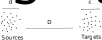
\includegraphics[width=0.5\textwidth]{introduction/degenerate_kernel.pdf}
    \caption{A set of source and target particle cluster, where the width of each cluster is significantly less than the distance separating them, $d_s, d_t \ll D$.}
    \label{fig:chpt:fmm:degenerate_kernel}
\end{figure}

Naively computed this requires $O(MN)$ operations. The \acrshort{fmm} relies on a \textit{degenerate} approximation of the interaction kernel when clusters of source and target particles are sufficiently separated, as sketched in Figure \ref{fig:chpt:fmm:degenerate_kernel}. Following the discussion in \cite{kailasa2024m2ltranslationoperatorskernel} the sum (\ref{eq:chpt:fmm:laplace_potential_sum}) can be written as,

\begin{equation}
    \phi(\mathbf{x}_i) \approx \sum_{p=1}^P \sum_{j=1}^N A_p(\mathbf{x}_i) B_p(\mathbf{y}_j)q(\mathbf{y}_j), \> \> i = 1,...,M
    \label{eq:chpt:introduction:sec:motivation:degenerate_kernel}
\end{equation}

where we call $P$ the expansion order, taken such that $P \ll N$, $P \ll M$. The functions $A_p$ and $B_p$ are defined by the approximation scheme used by a particular approach for the \acrshort{fmm}, in the original presentation the calculation,

\begin{equation}
    \hat{q}_p = \sum_{j=1}^N B_p(\mathbf{y}_j)q(\mathbf{y}_j)
\end{equation}

Corresponded to the coefficients of an order $P$ multipole expansion due to the source charges. Following which the potential is approximated by,

\begin{equation}
    \phi(\mathbf{x}_i) \approx \sum_{p=1}^P A_p(\mathbf{x}_i)\hat{q}_p, \> \> i = 1,...,M
\end{equation}

at the target particles. The approximation of the potential with this scheme can be seen to require $O(P(M+N))$ operations. The accuracy of this approximation scheme, and the error bounds provided by the \acrshort{fmm}, depends on the distance between the source and target clusters remaining large relative to their width. This condition is often referred to as an \textit{admissibility condition} in the \acrshort{fmm} literature. \acrshort{fmm}s therefore split the sum (\ref{eq:chpt:fmm:laplace_potential_sum}) into \textit{near} and \textit{far} components when considering arbitrary clusters of source and target particles,

\begin{equation}
    \phi(\mathbf{x}_i) = \sum_{\mathbf{y}_j \in \text{Near}(\mathbf{x}_i)} K(\mathbf{x}_i, \mathbf{y}_j) q(\mathbf{y}_j) +  \sum_{\mathbf{y}_j \in \text{Far}(\mathbf{x}_i)} K(\mathbf{x}_i, \mathbf{y}_j) q(\mathbf{y}_j), \> \> i=1,..,M
\end{equation}

In cases where a source and target cluster can be considered \textit{admissable}, i.e. the source cluster is considered in the \textit{far field} of the target cluster such that each $\mathbf{y}_j \in \text{Far}(\mathbf{x}_j)$, we apply the approximation (\ref{eq:chpt:introduction:sec:motivation:degenerate_kernel}). However, when a source and target cluster are \textit{inadmissable}, such that the source cluster is considered in the \textit{near field} of a target cluster such that each $\mathbf{y}_j \in \text{Near}(\mathbf{x}_j)$ we are left to evaluate the sum directly via (\ref{eq:chpt:fmm:laplace_potential_sum}).

In order to achieve its $O(N)$ complexity the FMM is structured to reduce to a minimum the number of sums evaluated between inadmissable clusters. This is achieved with a hierarchical discretisation of the problem domain, often a \textit{quadtree} in two dimensions and correspondingly an \textit{octree} in three dimensions. These data structures are generated by creating a bounding box that covers the source and target particles, which without loss of generality may correspond to the same set. This box is then recursively sub-divided into \textit{child boxes} of equal size.

- Overview of FMM algorithm for non-Oscillatory kernels.

- A brief not on computing changes in the past decades, and which part of the algorithm are a little redundant.

- A reflection on the key hidden constants in complexity, and why this may no longer be the most significant factor in modern implementations.

- A note on FMM software that is available, its positives and negatives, and why this is a little different.

- Conclude with why this thesis exists, to tackle these problems.
